\documentclass[review]{elsarticle}

\usepackage{lineno,hyperref}
\modulolinenumbers[5]

\journal{Journal of \LaTeX\ Templates}

%%%%%%%%%%%%%%%%%%%%%%%
%% Elsevier bibliography styles
%%%%%%%%%%%%%%%%%%%%%%%
%% To change the style, put a % in front of the second line of the current style and
%% remove the % from the second line of the style you would like to use.
%%%%%%%%%%%%%%%%%%%%%%%

%% Numbered
%\bibliographystyle{model1-num-names}

%% Numbered without titles
%\bibliographystyle{model1a-num-names}

%% Harvard
%\bibliographystyle{model2-names.bst}\biboptions{authoryear}

%% Vancouver numbered
%\usepackage{numcompress}\bibliographystyle{model3-num-names}

%% Vancouver name/year
%\usepackage{numcompress}\bibliographystyle{model4-names}\biboptions{authoryear}

%% APA style
%\bibliographystyle{model5-names}\biboptions{authoryear}

%% AMA style
%\usepackage{numcompress}\bibliographystyle{model6-num-names}

%% `Elsevier LaTeX' style
\bibliographystyle{elsarticle-num}
%%%%%%%%%%%%%%%%%%%%%%%

\begin{document}

\begin{frontmatter}

\title{Atrial Fibrillation Detection from Short-Term Recording of a Single Abduction}
	% \LaTeX\ template\tnoteref{mytitlenote}}
\tnotetext[mytitlenote]{Fully documented templates are available in the elsarticle package on \href{http://www.ctan.org/tex-archive/macros/latex/contrib/elsarticle}{CTAN}.}

%% Group authors per affiliation:
%\author{Asiminidis Christodoulos\fnref{myfootnote}}
%\address{Imperial College London, United Kingdom}
%\fntext[myfootnote]{Since 1880.}

%% or include affiliations in footnotes:
%\author[chasiminidis@cs.uoi.gr, +306986076324, +35797758931]{Elsevier Inc}
%\ead[url]{www.elsevier.com}

%\author[mysecondaryaddress]{Global Customer Service\corref{mycorrespondingauthor}}
%\cortext[mycorrespondingauthor]{Corresponding author}
%\ead{support@elsevier.com}
%
%\address[mymainaddress]{1600 John F Kennedy Boulevard, Philadelphia}
%\address[mysecondaryaddress]{360 Park Avenue South, New York}

\begin{abstract}
Atrial Fibrillation has always been on the spotlight in the academic research part firstly in medical sciences and therefore, based on technological advancements, in computer sciences as well. It is type of heart beat rate inconsistency in which the human body's heart rate does not function as most of the human's heart beats do. It affects a very small part of the mankind globally, around 1.5\%, but its consequences are very serious. This work focuses on the detection and therefore prediction of atrial fibrillation heart beats. At first, atrial fibriallation is explained, giving an example, the dataset is described which consists of four different types of heart beat rates and thereafter the results and outcomes are presented.
% \LaTeX\ manuscript.
\end{abstract}

\begin{keyword}
\texttt{Atrial Fibrillation} \sep Short-Term Recording
\sep Single Abduction
\sep Multi-class classification supervised machine learning model 
\sep Model Accuracy
%\MSC[2010] 00-01\sep  99-00
\end{keyword}

\end{frontmatter}

\linenumbers

\section{Introduction}

%\paragraph{Installation}
% If the document class \emph{elsarticle} is not available on your computer, you can download and install the system package \emph{texlive-publishers} (Linux) or install the \LaTeX\ package \emph{elsarticle} using the package manager of your \TeX\ installation, which is typically \TeX\ Live or Mik\TeX.

ECG examinations firstly appeared back the 19th century. Willem Eingthofen was the first one who proposed and received the Nobel Prize in 1924. ECG is a way to examine and diagnose heart beat rates and does not actually by no means interfere into the human body. It helps diagnose the normal heart beat rate like stroke, dementia, anomalies and fibrillations \cite{puniaElectrographicClinicalNatural2017, staerkAtrialFibrillation2017}. 
An ECG is based on measurements emphasizing the P, Q, R, S, T curve spots. The results extracted from an ECG define the conditions and the situation in which the patient is currently in. For example, results are currently based on the season. People who are in charge, especially mostly and hopefully only doctors in this case acknowledge the fact that the ECG received presents an ECG illustration susceptible to mistakes, computer-wised such as noise \cite{osmanElectrographicPredictorsElectrographic2018, lippiGlobalEpidemiologyAtrial2021, chuaDynamicChangesCardiovascular2021} due to computer, accuracy error.

Figure \ref{fig:NormalECG} illustrates  a heart input, the so-called Atreus in which contractions happen and the blood flows from the inner part into the ventricular system. R-wave is the ventricular system in which there are two large inputs of repolarization that creates the central circulatory system. T-wave is step right before of the heart repolarization that happens in order to restart the heart rate and the next heart beat comes forward clock-wise. 
The time being between the P-wave and the QRS complex is the time that before the advent of the heart contraction atrium up until the heart ventricle. The particular time is named after P-Q period of time. Well, the normal P-Q period of time is all but 0.16 seconds. That period of time is sometimes called P-R because there are times when Q is absent. 
The ventricle contraction practically leads from the start of Q wave up until the end of T wave. That period of time is named after Q-T  of time and the normal period of time is 0.35 seconds. 
The frequency of heart beat rate is defined easily from an ECG instance, because that period of time that interference between two consecutive heart beats is the inverse of the heart frequency. If the period of time that interferes between two consecutive heart beats, as defined with enumeration lines, is equal to 1 second, the heart frequency is equal to 60 heart beats per minute. The normal period of time that interferes between QRS complex is equal to 0.83 seconds. Therefore, this heart frequency in this case is equal to 72 heart beats per minute. 
Heart beat fibrillation are classified based on originality, beat, period of time and/or creation mechanism. The originality category is classified into ventricular fibrillation, ventricle fibrillation and fibrillation that origins from AV circularity. The heart beat is classified in bradycardia (rate $\leq$ 60 beats/min) and tachycardia (rate $\geq$ 100 beats/min). The period of time is clssified into the chronic heart beat ($\ge$ 30 seconds) and the non-chronic one ( $\leq$ 30 seconds). The creation and the beginning of a heart rate is classified into the polarization starts automatically without cells being bother one another, metapolarization in which primary polarization leads into emergent contractions due to elecrical instability into the membrane and reentering in which the current follows a circular movement and repolarizes circularly the cells that have been polarized \ref{fig:boat1}. 

\begin{figure}
	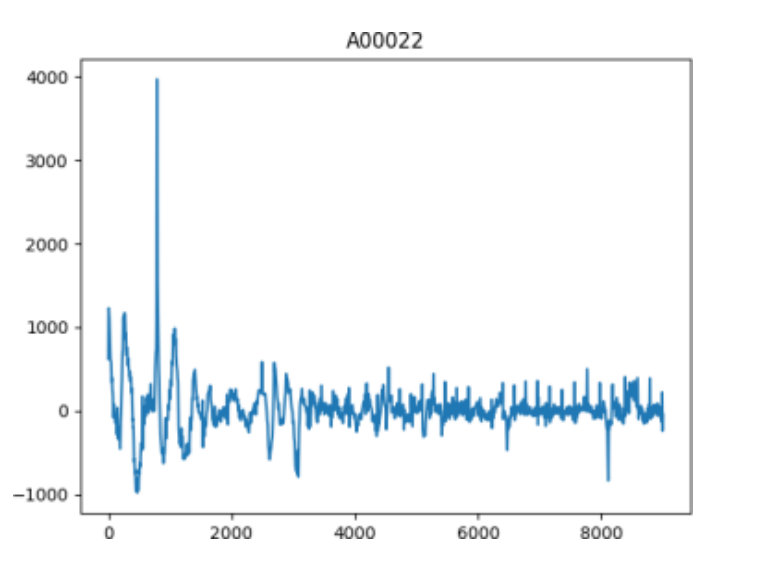
\includegraphics[width=50mm,scale=0.5]{Figures/Noise.png}
	\centering
	\caption{ECG presenting Noise.}
	\label{fig:boat1}
\end{figure}

%\paragraph{Usage} Once the package is properly installed, you can use the document class \emph{elsarticle} to create a manuscript. Please make sure that your manuscript follows the guidelines in the Guide for Authors of the relevant journal. It is not necessary to typeset your manuscript in exactly the same way as an article, unless you are submitting to a camera-ready copy (CRC) journal.
%
%\paragraph{Functionality} The Elsevier article class is based on the standard article class and supports almost all of the functionality of that class. In addition, it features commands and options to format the
%\begin{itemize}
%\item document style
%\item baselineskip
%\item front matter
%\item keywords and MSC codes
%\item theorems, definitions and proofs
%\item lables of enumerations
%\item citation style and labeling.
%\end{itemize}

\section{Atrial Fibrillation}
Atrial Fibrillation is the most ordinary heart beat inconsistent form. It appears to 1-2 \% of the total worldwide. Nowadays, almost 12 million Europeans and Americans are diagnosed with urgent Atrial Fibrillation. Atrial Fibrillation increases as long as human being ages. It hardly is diagnosed because it is sudden. Figure \ref{fig:ExampleAtrialFibrillationandNormalOne} illustates two graphs in which the first one presents the pattern of the heart beat progress along with normal heart beat and the second one on the bottom of the graph presents an ECG instance diagnosed with Atrial Fibrillation. X-axis shows time in seconds and y-axis shows Amplitude in mV.

\begin{figure}[h!]
	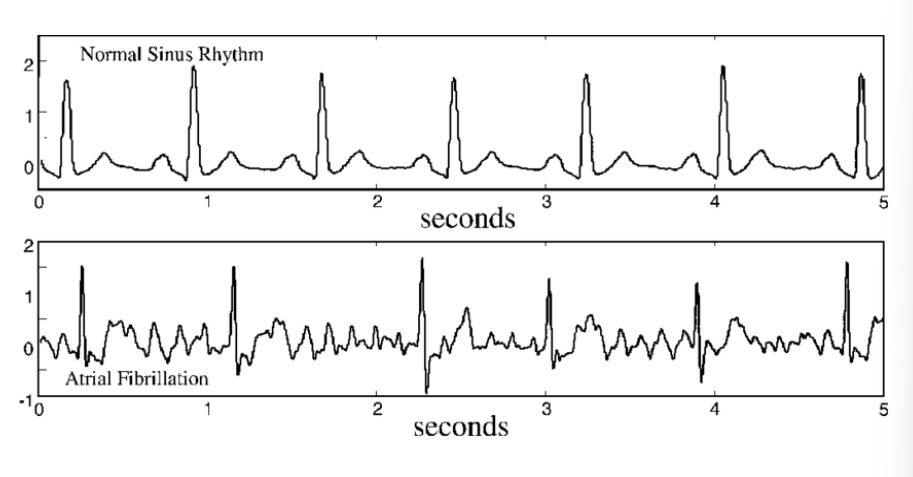
\includegraphics[width=50mm,scale=0.5]{./Figures/ExampleAtrialFibrillationandNormalOne.png}
	\centering
	\caption{Normal ECG Example with wave representations}
	\label{fig:ExampleAtrialFibrillationandNormalOne}
\end{figure}

The goal of this work is dataset classification based on heart beat rate using classification supervised machine learning methods which is one of the machine learning model categories. There are four different heart beat categories, the first one is the normal one (N), the second one is the one of Atrial Fibrillation (A), a random noise (O) and noise (~). The given, corresponding data set consists of 8.528 instances and they are patient recordings. They are publicly available for a contest that took place in 2017 for the dataset training part using machine learning methods for the best accuracy model extraction to predict the heart beat type \cite{linkerAccurateAutomatedDetection2016}. 


%
%The author names and affiliations could be formatted in two ways:
%\begin{enumerate}[(1)]
%\item Group the authors per affiliation.
%\item Use footnotes to indicate the affiliations.
%\end{enumerate}
%See the front matter of this document for examples. You are recommended to conform your choice to the journal you are submitting to.

\section{Research Methodology}
In order to extract a classification machine learning model, our data first and foremost should be analyzed and pre-processed. The data set consists of 8.528 instances. Each one of the instance belongs to one of the four classes, in total. The annotation of each class is as follows. The letter N corresponds to the class in which the heart rate is normal, the letter A corresponds to the class in which the heart rate belongs to the one classified as atrial fibrillation, the letter O corresponds to the class in which the heart rate belongs to an arbitrary heart rate and the $\tilde{}$ corresponds to the class in which there is noise in the ECG sample-instance examined.
One of the basic steps of pre-processing is to find the total number of observations that corresponds to each of the four classes. Firstly, classes have been decoded in a computer-wise manner. The class with the letter A takes the value of 0, the class N takes the value 1, the class O takes the value of 2 and the class that corresponds to the letter $\tilde{}$ takes the value 3. 


\begin{figure}[h!]
	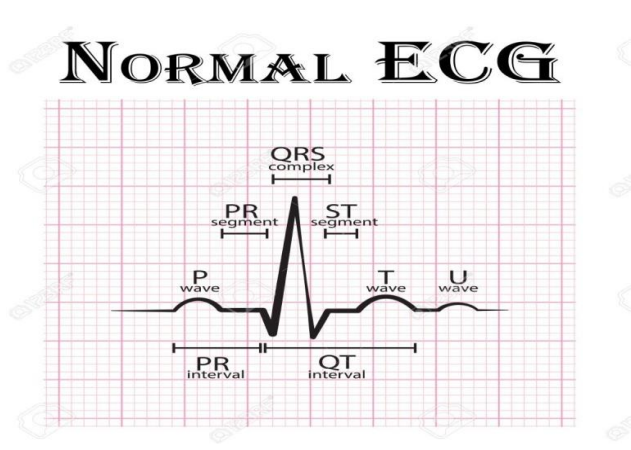
\includegraphics[width=50mm,scale=0.5]{./Figures/NormalECG.png}
	\centering
	\caption{Normal ECG Example with wave representations}
	\label{fig:NormalECG}
\end{figure}


%\section*{Figures}
\begin{figure}[h!]\label{Normal_Heart_Rate}
	\caption{Normal Heart Rate}
\end{figure}

%\section*{Figures}
\begin{figure}[h!]
	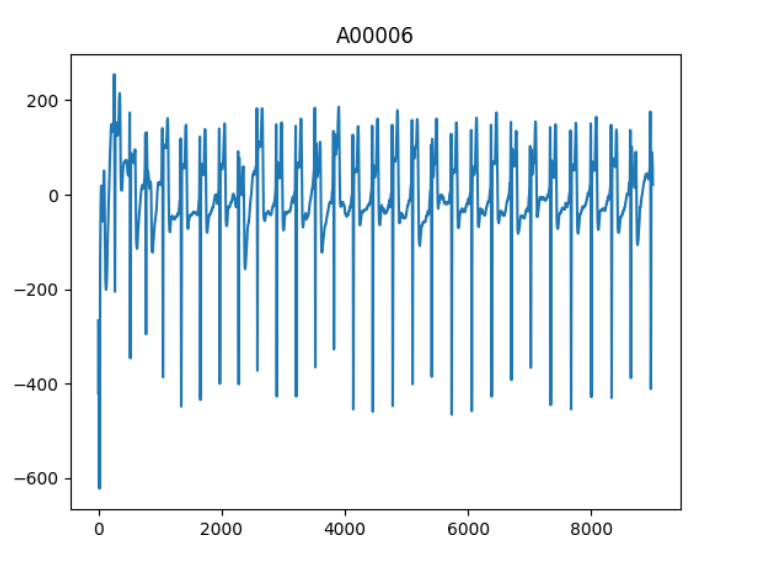
\includegraphics[width=50mm,scale=0.5]{./Figures/NormalHeartRate.png}
	\centering
	\caption{Normal Heart Rate}
	\label{fig:NormalHeartRate}
\end{figure}


\begin{figure}[h!]
	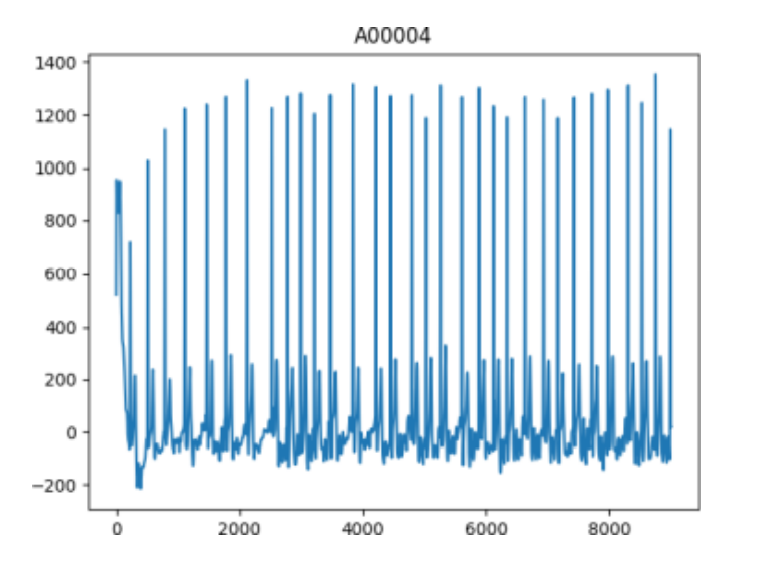
\includegraphics[width=50mm,scale=0.5]{./Figures/AtrialFibrillation.png}
	\centering
	\caption{Atrial Fibrillation}
	\label{fig:AtrialFibrillation}
\end{figure}

\begin{figure}[h!]
	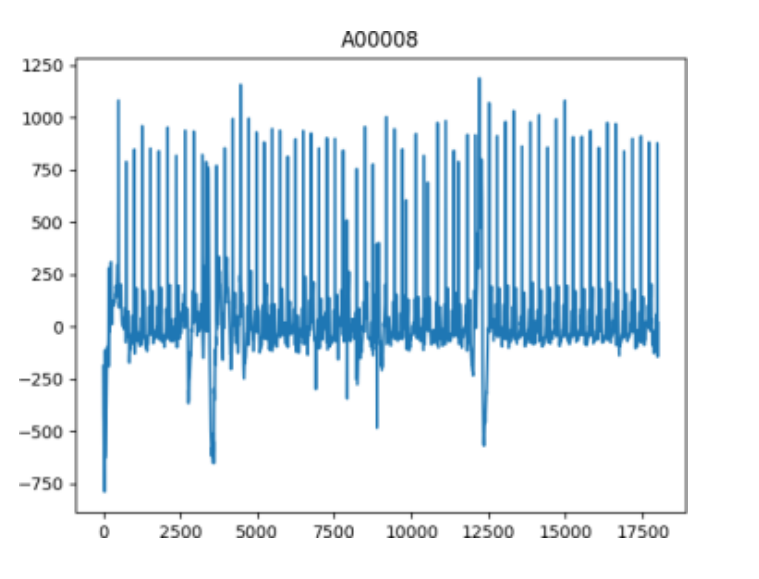
\includegraphics[width=50mm,scale=0.5]{./Figures/ArbitraryHeartRate.png}
	\centering
	\caption{Arbitrary Heart Rate}
	\label{fig:ArbitraryHeartRate}
\end{figure}

\begin{figure}[h!]
	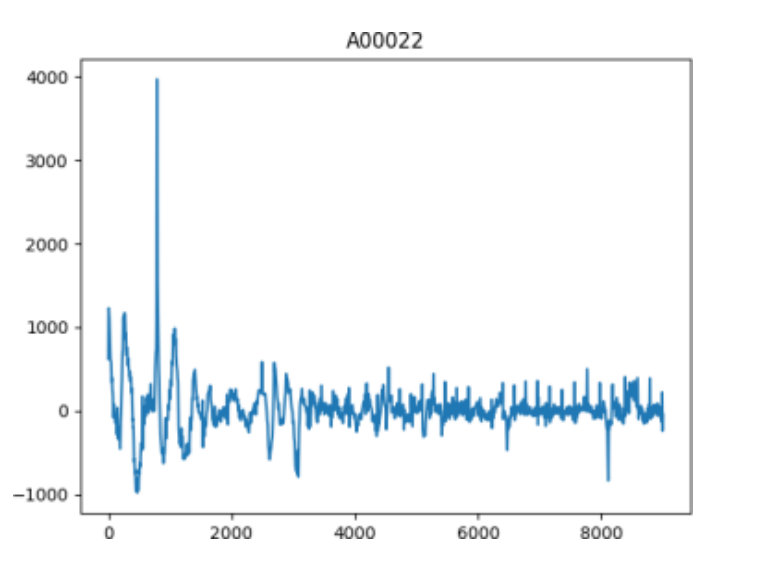
\includegraphics[width=50mm,scale=0.5]{./Figures/Noise.png}
	\centering
	\caption{Noise}
	\label{fig:Noise}
\end{figure}


The given data set is imbalanced, according to Table \ref{tab:imbalanceddatasetenumeration}. That means that there is skewness in the data classification. Specifically, the proportion of the observations, instances of the class that corresponds to the letter N and the class that corresponds to the class with the symbol $\tilde{}$ is 1:18.

%\section*{Tables}
\begin{table}[h!]
	\caption{Imbalances dataset enumeration \label{tab:imbalanceddatasetenumeration}}
	\centering
	\begin{tabular}{cc}
		\hline
		Class & No. of Observations \\ \hline
		'A' & 738 \\
		'N' & 5050 \\
		'O' & 2456 \\
		'$\tilde{}$' & 284 \\ \hline
		
	\end{tabular}
	
\end{table}

In order to face the imbalance data into our data set, the particular framework oversamples the sample, meaning that it dupliactes the instances from the class which has the least number of observations into the training data set. The goal is to avoid any error caused because out model is about to overfit. In order to solve such issues, the reduction or even the removal of some instances from the classes that might have more observations than the ones which have less, so that the number of observations is close or the same with the one which has more instances. Therefore, the data set consists of 1.136 instances in which each class has equal number of observations corresponding to 285 observations. 

The second number of observations of preprocessing is the removal of continuous current that is created into the ECG instance examination.  So, in order to make sure that there is such a noise from the power supply, DC bias is calculated which gives the mean of each wavelength. If the mean of each wavelength equals to zero, then there is no DC bias. In this particular case, there is DC bias and there will always be on most of the cases. In order to deal with such a preprocessing data cleaning, the mean of each ECG is calculated and subsequently, the values are normalized in the range of between -1 and 1, [-1,1]. 

The third step is the feature extraction through the ECG cardiographs. Using the appropriate libraries in Python programming language such as scipy and biosppy and in accordance with the help of basic mathematical calculations such as mean, median, minimum and maximum values. The calculation of the feature extraction outputs the following features from the medical point of view. PR interval shows the time between the starting point of P-wave up until the starting point of QRS curve, the maximum value of P-wave, time between P and R waves, time between P and W, the part between ST curves, the maximum value of T, a value corresponding before the maximum value of R wave, a value corresponding after the maximum value of R wave, the time being between T and R waves, time between T and S waves, time between P and T waves, skewness in P wave, curve in T wave, time being in QRS curves, time being in QS curves, kurtosis in QRS, skewness in QRS and the difference between the maximum and the minimum value of QRS wave that appears in an ECG instance. 

Data pre-processing task is completed and therefore, the implementation and evaluation of machine learning model in \ref{sec:ResearchOutcomes}.

%\nameref{section:ResearchOutcomes}.


\section{Research Analysis and Preprocessing metrics}\label{sec:ResearchOutcomes}
The particular machine learning used belongs to a classification supervised machine learning categories. A lof ot applications in machine learning are based on multi-class classification models. The challenge and work examined in this paper belongs to multi-class classification machine learning models because the number of classes supervised is greater than 1.

So, in a binary classification problem, there are two classes often called P and N, named after Positive and Negative. In such a problem, the confusion matrix extraction is a good tactic, in which there are two rows and columns respectively. In multi-class classification problem such that, the terms of Precision and Recall are presented. Precision term is referred to True Positive quantity divided by the addition of True and False Positive. From the mathematical point of view, Precision metric is described as follows \ref{precisionmathematicalform}:


\begin{equation}\label{precisionmathematicalform}
		Precision  = \frac{TP}{TP + FP}
\end{equation}

Precision metric shows the proportion of the predicted values which are truly positive and not predicted as false though they were true. 
A second metric examine is the Recall metric. This particular, mathematically speaking, is expressed in \ref{recallmathematicalform}.

\begin{equation}\label{recallmathematicalform}
		Recall = \frac{TP}{TP + FN}
\end{equation}

The Recall metric is referred to True Positive divided by the addition of the ones which are True Positive and False Negative. Recall metric covers the question of the proportion of the True Positive are correctly classified as given in \ref{accuracymathematicalform}. 

\begin{equation}\label{accuracymathematicalform}
		Accuracy = \frac{TP + TN}{TP + TN + FP + FN}
\end{equation}

So, it is the summation of the diagonal values of the confusion matrix divided by the total values of the matrix.

An additional metric that needs to be mentioned is the F1-score. This particular metric outputs a value between Precision and Recall metrics. It is not considered a reliable one, though many researcher still use it to compare machine learning models \cite{f1score}. F1-score is expressed in equation \ref{f1scoremetric}.

\begin{equation}\label{f1scoremetric}
		F1_score = 2 \times \frac{precision*recall}{precision + recall}
\end{equation}

The reason that the particular metric won't be taken into consideration is because it emphasizes mostly on lower values that Precision and Recall metrics output. For instance, if Precision is 100\% and Recall 0\%, then F1\-score equals to 0\% and not 50\%. 

The machine learning model studies, examined and implemented belongs to supervised machine learning models and is the Random Forest one. Shortly, decision trees from the given data set are created so that the decision is taken into consideration from each one of them. The Random Forest algorithm samples a particular number of instances from the current data set. The algorithm constructs a decision tree for each sample and receives an output from each of these samples. Each sample output is configured whether it is an appropriate one or not for classification prediction. 

Experiments have been conducted successfully adjusting the appropriate parameters of the machine learning models so that the best optimal accuracy is succeeded and as a result, the selection of the best machine learning model. The best optimal result is chosen with the one that consists of the most final predicted/supervised summation output.

Machine learning training processed had been performed firstly tuning the hyperparameters of the machine learning model so that the best accuracy score succeeded and consequently the best model is chosen. There are three metrics examined for the evaluation and the comparison amongst these models. The metrics are the Mean Absolute Error (MAE), Mean Squared Error(MSE) and Root Mean Squared Error (RMSE). Mean Absolute Error (MAE) is mathematically described in equation \ref{meanabsoluteerror}.

\begin{equation}\label{meanabsoluteerror}
		% F1_score = 2 \times \frac{precision*recall}{precision + recall}
		MAE = \sum_{i=1}^{n} \frac{||y_{i} - \lambda(x_{i})||}{n}
\end{equation}


Mean Squared Error is described in equation \ref{meansquarederror}.

\begin{equation}\label{meansquarederror}
		% F1_score = 2 \times \frac{precision*recall}{precision + recall}
		% MAE = \sum_{i=1}^{n} \frac{||y_{i} - \lambda(x_{i})||}{n}
		MSE = \frac{1}{n} \times \sum_{i=1}^{n} (y_{i} - \lambda(x_{i}))
\end{equation}

Root Mean Square Error is described in equation \ref{rootmeansquareerror}.


\begin{equation}\label{rootmeansquareerror}
		\sqrt{\frac{\sum_{i=1}^{n} (y_{i} - \lambda\times(x_{i}))}{n}}
		%\sum_{i=}^{max}
		% F1_score = 2 \times \frac{precision*recall}{precision + recall}
		% MAE = \sum_{i=1}^{n} \frac{||y_{i} - \lambda(x_{i})||}{n}
		%MSE = \frac{1}{n} \times \sum_{i=1}^{n} (y_{i} - \lambda(x_{i}))
\end{equation}

in which n shows the total number of the sample of y\_{i} which shows the real ones and $\lambda$  %(x\_{i}).

\section{Research outcomes}
The parameters in which the evaluation of the model is considered and subsequently the accuracy score of the particular work is estimated to be the number of the decision trees of the Random Forest algorithm (n\_estimators) and the minimum number of the sample at each leaf of the random forest. It is considered that the weight of the leaves is equal to all of them.


So, starting and setting n\_estimators = 10 and the number of leaves in the decision trees is from 1 to 10, the best optimal model is about to the one in which the number of leaves is equal to 3. Table \ref{matricresultsnestimators10} displays the results with the best optimal number of leaves in the decision tree to be equal to 3 which the errors are the following ones MAE = 0.51, MSE = 0.97, RMSE = 0.99 and Accuracy Score 0.69. 

\begin{table}[h!]
	\caption{Metric results for n\_estimators = 10 \label{matricresultsnestimators10}}
	\centering
	\begin{tabular}{ccccc}
		\hline
		Leaf & MAE \ref{meanabsoluteerror} & MSE \ref{meansquarederror} & RMSE \ref{rootmeansquareerror} & Accuracy Score \ref{accuracymathematicalform}\\ \hline
		1 & 0.62 & 1.23 & 1.11 & 0.63\\
		2 & 0.54 & 1.06 & 1.03 & 0.68 \\
		3 & \b{0.53} & \b{1.04} & \b{1.02} & \b{0.69} \\
		4 & 0.59 & 1.15 & 1.07 & 0.64\\
		5 & 0.56 & 1.09 & 1.04 & 0.67\\
		6 & 0.61 & 1.22 & 1.10 & 0.64\\
		7 & 0.60 & 1.18 & 1.09 & 0.64\\
		8 & 0.61 & 1.20 & 1.10 & 0.65\\
		9 & 0.58 & 1.15 & 1.07 & 0.66\\
		10 & 0.63  & 1.23 & 1.11 & 0.63\\ \hline
	\end{tabular}
\end{table}

For n\_estimators = 10 and the number of leaves in the decision tree starting from 1 to 10, the best optimal number of leaves for the decision tree equals to 3. Table \ref{matricresultsnestimators100} shows the results for the best optimal number of leaves equals to 3 in which the errors are the following ones, MAE $\equiv$ 0.51, MSE $\equiv$ 0.97 and RMSE $\equiv$ 0.99.

\begin{table}[h!]
	\caption{Metric results for n\_estimators = 100 }
	\centering
	\label{matricresultsnestimators100}
	\begin{tabular}{ccccc}
		\hline
		Leaf & MAE \ref{meanabsoluteerror} & MSE \ref{meansquarederror} & RMSE \ref{rootmeansquareerror} & Accuracy Score \ref{accuracymathematicalform}\\ \hline
		1 & 0.54 & 1.09 & 1.05 & 0.69 \\
		2 & 0.52 & 0.99 & 1.00 & 0.69 \\
		3 & 0.51 & 0.97 & 0.99 & 0.69 \\
		4 & 0.53 & 1.02 & 1.01 & 0.68 \\
		5 & 0.53 & 1.03 & 1.01 & 0.68 \\
		6 & 0.56 & 1.08 & 1.04 & 0.67 \\
		7 & 0.55 & 1.05 & 1.02 & 0.67 \\
		8 & 0.55 & 1.07 & 1.03 & 0.67 \\
		9 & 0.56 & 1.11 & 1.06 & 0.68 \\
		10 & 0.55  & 1.05 & 1.02 & 0.67 \\ \hline
	\end{tabular}
\end{table}


For n\_estimators = 1.000 and for the number of leaves in the decision tree starting from 1 to 100, the best optimal number of leaves in the decision tree equals to 5. Table \ref{label} displays the results with the best optimal number of leaves in the decision tree to be equal to 5 which the errors are the following ones MAE $\equiv$ 0.55, MSE $\equiv$ 1.07 and RMSE $\equiv$ 1.04. 

\begin{table}[h!]
	\caption{Metric results for n\_estimators = 1000 }
	\centering
	\label{matrixresultsnestimators1000}
	\begin{tabular}{ccccc}
		\hline
		Leaf & MAE \ref{meanabsoluteerror} & MSE \ref{meansquarederror} & RMSE \ref{rootmeansquareerror} & Accuracy Score \ref{accuracymathematicalform}\\ \hline
		1 & 0.55 & 1.08 & 1.04 & 0.68 \\
		2 & 0.55 & 1.09 & 1.04 & 0.67 \\
		3 & 0.57 & 1.11 & 1.05 & 0.67 \\
		4 & 0.55 & 1.11 & 1.05 & 0.68 \\
		5 & 0.55 & 1.07 & 1.04 & 0.68 \\
		6 & 0.56 & 1.11 & 1.05 & 0.67 \\
		7 & 0.57 & 1.12 & 1.06 & 0.66 \\
		8 & 0.56 & 1.10 & 1.05 & 0.67 \\
		9 & 0.57 & 1.11 & 1.05 & 0.66 \\
		10 & 0.56  & 1.09 & 1.04 & 0.66 \\ \hline
	\end{tabular}
\end{table}


For n\_estimators = 10.000 and for the number of leaves in decision tree starting from 1 to 10, the best optimal number of leaves for the decision tree equals to 9. In table \ref{matrixresultsnestimators10000} shows the results with the best optimal number of leaves to be equal to 9 with the following errors, MAE $\equiv$ 0.55, MSE $\equiv$ 1.06 and RMSE $\equiv$ 1.03. 

\begin{table}[h!]
	\centering
	\caption{Metric results for n\_estimators = 10000 }
	\label{matrixresultsnestimators10000}
	\begin{tabular}{ccccc}
		\hline
		Leaf & MAE \ref{meanabsoluteerror} & MSE \ref{meansquarederror} & RMSE \ref{rootmeansquareerror} & Accuracy Score \ref{accuracymathematicalform}\\ \hline
		1 & 0.55 & 1.07 & 1.03 & 0.67 \\
		2 & 0.56 & 1.08 & 1.04 & 0.67 \\
		3 & 0.57 & 1.11 & 1.05 & 0.67 \\
		4 & 0.57 & 1.11 & 1.06 & 0.66 \\
		5 & 0.56 & 1.09 & 1.04 & 0.67 \\
		6 & 0.55 & 1.08 & 1.04 & 0.67 \\
		7 & 0.55 & 1.08 & 1.04 & 0.67 \\
		8 & 0.56 & 1.10 & 1.05 & 0.67 \\
		9 & 0.55 & 1.06 & 1.03 & 0.67 \\
		10 & 0.55  & 1.07 & 1.03 & 0.67 \\ \hline
	\end{tabular}
\end{table}


According to Tables \ref{matricresultsnestimators10}, \ref{matricresultsnestimators100}, \ref{matrixresultsnestimators1000}, \ref{matrixresultsnestimators10000} which correspond to the best optimal results based pn the calculated errors. Table \ref{bestresultsmaemsermse} shows that the best machine learning model is equal to the number of trees to be equal to 100 and the number of leaves of the decision tree to be equal to 3.

\begin{table}[h!]
	\caption{Best results of MAE, MSE and RMSE}
	\centering
	\label{bestresultsmaemsermse}
	\begin{tabular}{ccccc}
		\hline
		Leaf & n\_estimators & MAE \ref{meanabsoluteerror} & MSE \ref{meansquarederror} & RMSE \ref{rootmeansquareerror} \\ \hline
		3 & 10 & 0.53 & 1.04 & 1.02 \\
		3 & 100 & 0.51 & 0.97 & 1.00 \\
		5 & 1000 & 0.55 & 1.07 & 1.04 \\
		9 & 10.000 & 0.55 & 1.06 & 1.03 \\ \hline
	\end{tabular}
\end{table}

The next step is the confusion matrix extraction to be estimated accurately: \newline
$\bullet$ signal that have already been categorized as Atrial Fibrillation compared with the ones categorized as normal and  \newline
$\bullet$ signals that have already been categorized as Atrial Fibrillation compared with the ones categorized that they do not belong to the Atrial Fibrillation category. 

Table \ref{confusionmatrix} shows the confusion matrix results.

\begin{table}[h!]
	\caption{Confusion Matrix}
	\centering
	\label{confusionmatrix}
	\begin{tabular}{ccccc}
		\hline
		& A & N & O & $\tilde{}$ \\ \hline
		A & 63 & 0 & 11 & 10 \\
		N & 2 & 52 & 13 & 7 \\
		O & 25 & 21 & 39 & 8 \\
		$\tilde{}$ & 1 & 3 & 5 & 81 \\ \hline
	\end{tabular}
\end{table}


Rows horizontally represent the predicted values, whilst the columns vertically represent the real ones.

Assuming it was a binary classification, meaning that we only predicted whether the ECG derives from Atrial Fibrillation data set or not, the numbers are as follows, TP= 52, FP = 0, TN = 63 and FN = 2, Precision = 1, Recall = 0.96 and Accuracy = 0.98. 

As a multi-class classification problem as it is, Precision = 0.75, Recall = 0.89 and Accuracy = 0.68. 

\section{Conclusions}
Atrial Fibrillation is defined to be as an atrial fibrillation in which the heart rate speed is not synchronized normally based on consecutive normal beats. That happens to 1-2\% of the total population and is relevant to mortality and morbidity. The goal of this work is to score based on accuracy metrics which they separately characterized as Atrial Fibrillation, normal ones and the ones that they don't belong to any of the class. 
Results have shown that the first binary classification category reaches an accuracy score of 98\% , whilst the second multi class one reaches up to 68\%. The difference between these two cases is equal to 30\%. That difference is expected because, in the first case the machine learning model is a binary supervised one that belongs to Random Forest category and in the second case, the machine learning model is a multi class one that consist of four classes, the first one is the normal one, the second one is the atrial fibrillation one, the third one does not belong to any of the aforementioned classes and the last one is described as noise. 

%Text and results for this section, as per the individual journal's instructions for authors.
%
%\section*{Section title}
%Text for this section\ldots
%\subsection*{Sub-heading for section}
%Text for this sub-heading\ldots
%\subsubsection*{Sub-sub heading for section}
%Text for this sub-sub-heading\ldots
%\paragraph*{Sub-sub-sub heading for section}
%Text for this sub-sub-sub-heading\ldots
%
%In this section we examine the growth rate of the mean of $Z_0$, $Z_1$ and $Z_2$. In
%addition, we examine a common modeling assumption and note the
%importance of considering the tails of the extinction time $T_x$ in
%studies of escape dynamics.
%We will first consider the expected resistant population at $vT_x$ for
%some $v>0$, (and temporarily assume $\alpha=0$)
%%
%\[
%E \bigl[Z_1(vT_x) \bigr]=
%\int_0^{v\wedge
	%1}Z_0(uT_x)
%\exp (\lambda_1)\,du .
%\]
%%
%If we assume that sensitive cells follow a deterministic decay
%$Z_0(t)=xe^{\lambda_0 t}$ and approximate their extinction time as
%$T_x\approx-\frac{1}{\lambda_0}\log x$, then we can heuristically
%estimate the expected value as
%%
%\begin{equation}\label{eqexpmuts}
%\begin{aligned}[b]
%&      E\bigl[Z_1(vT_x)\bigr]\\
%&\quad      = \frac{\mu}{r}\log x
%\int_0^{v\wedge1}x^{1-u}x^{({\lambda_1}/{r})(v-u)}\,du .
%\end{aligned}
%\end{equation}
%%
%Thus we observe that this expected value is finite for all $v>0$ (also see \cite{koon,xjon,marg,schn,koha,issnic}).

%
%\section*{Appendix}
%Text for this section\ldots

%%%%%%%%%%%%%%%%%%%%%%%%%%%%%%%%%%%%%%%%%%%%%%
%%                                          %%
%% Backmatter begins here                   %%
%%                                          %%
%%%%%%%%%%%%%%%%%%%%%%%%%%%%%%%%%%%%%%%%%%%%%%

%\section{Bibliography styles}
%
%There are various bibliography styles available. You can select the style of your choice in the preamble of this document. These styles are Elsevier styles based on standard styles like Harvard and Vancouver. Please use Bib\TeX\ to generate your bibliography and include DOIs whenever available.
%
%Here are two sample references: \cite{Feynman1963118,Dirac1953888}.

%rences}

\bibliography{mybibfile}

\end{document}